\documentclass[xcolor=dvipsnames, 9pt]{beamer}
\usepackage{mathrsfs}
\usepackage{bm}
\usepackage{helvet}
\usepackage{graphicx}
\usepackage[english]{babel}
\usepackage[latin1]{inputenc}
\usepackage{times}
\usepackage[absolute]{textpos}
\setlength{\TPHorizModule}{\paperwidth}
\setlength{\TPVertModule}{\paperheight}

\setlength{\overfullrule}{2pt}
\usepackage{tikz}
\usetikzlibrary{snakes}
\usetikzlibrary{patterns}
\usetikzlibrary{arrows}

\usetheme{Frankfurt}
\useinnertheme{rounded}
\setbeamercovered{transparent}

\beamertemplatesolidbackgroundcolor{black!5}
\beamertemplatetransparentcovered

\newcommand{\greencol}{\color[RGB]{35,170,30}}
\setbeamerfont{bibfont}{size=\tiny}

\title{Design and Stabilization of a\\[0.05in]One Legged Hopper}
%\subtitle{Something catchy here}

\author[Pratik]{Pratik Chaudhari\\[0.1in]06D01015\\[0.3in]\small{Prof. Hemendra Arya\hfill Prof. Bhartendu Seth}\\[0.05in]\footnotesize{Guide\hspace{1.4in} Co-guide}}
\date{\footnotesize{B.Tech. Project}}

\AtBeginSection[]
{
    \begin{frame}<beamer>
		\frametitle{Outline}
        \small
        {
		    \tableofcontents[currentsection]
        }
	\end{frame}
}

\begin{document}
{
\usebackgroundtemplate{\begin{textblock}{0.6}(0.3,0.55)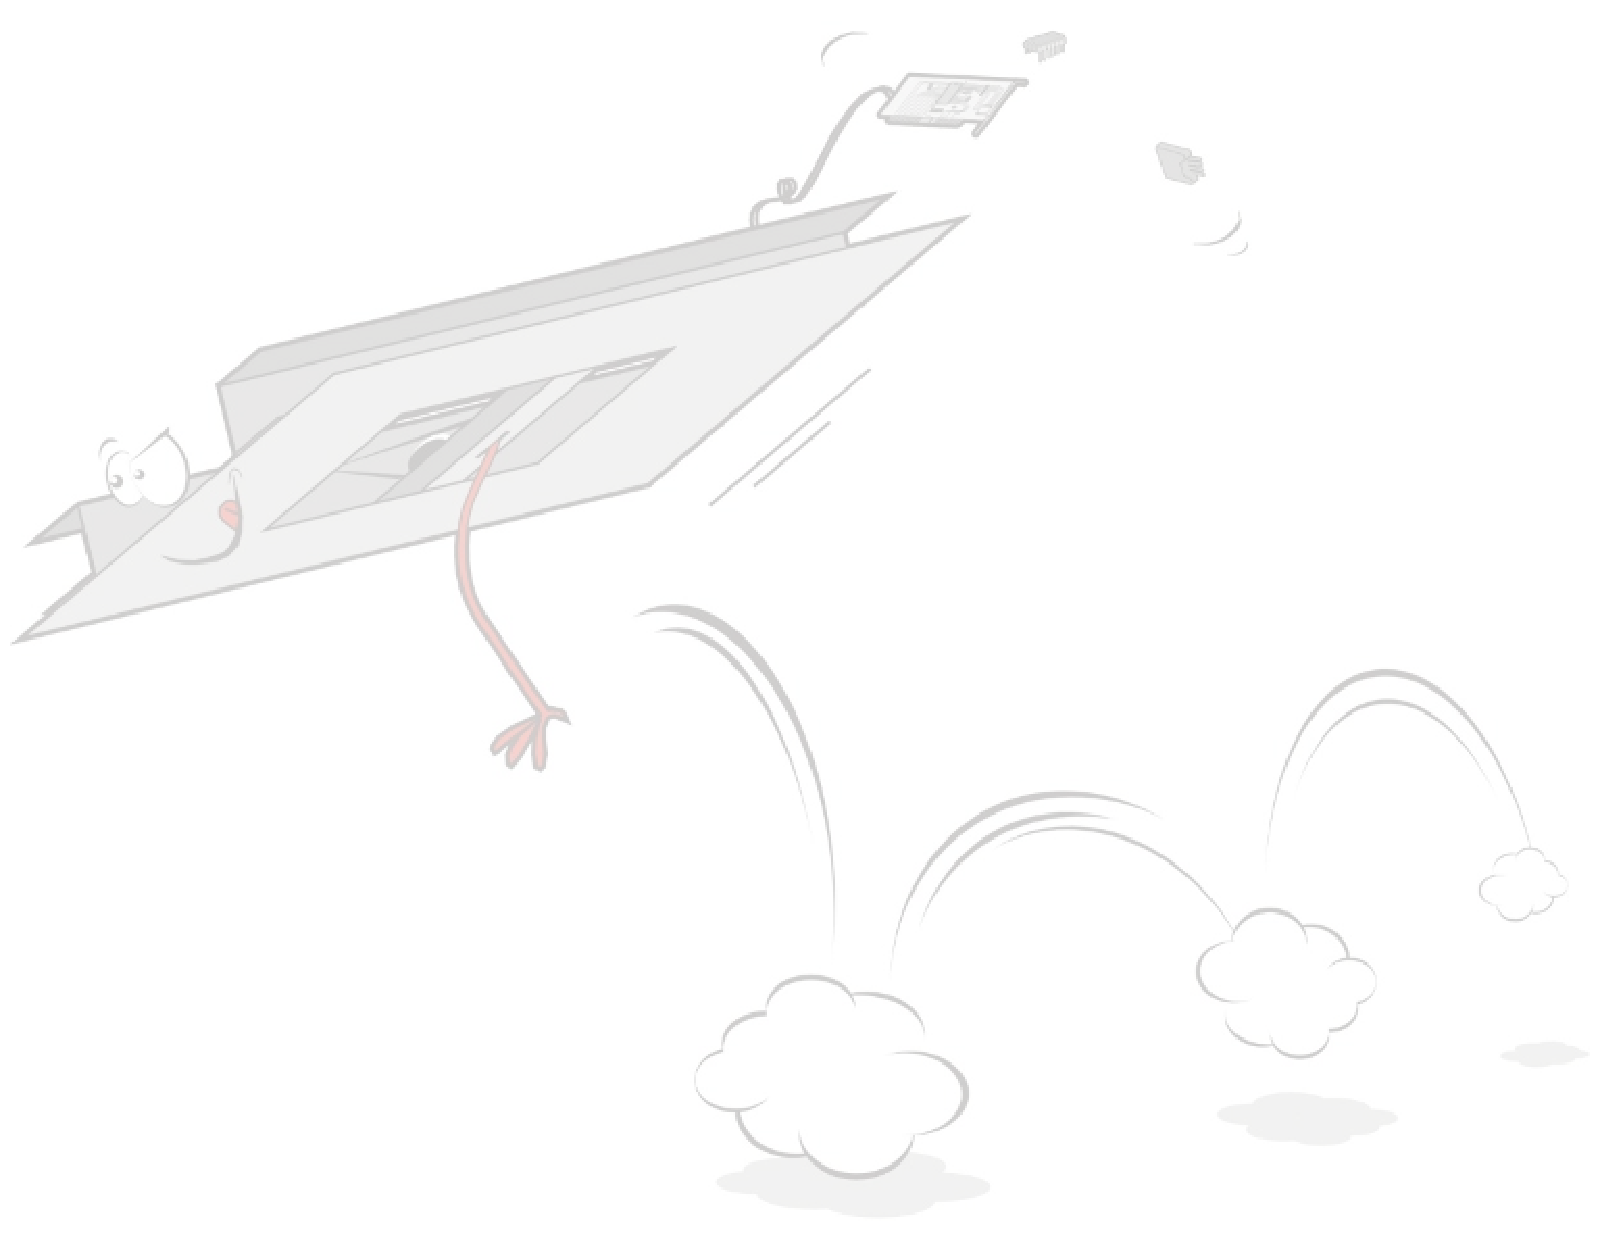
\includegraphics[scale=0.2]{fig/cartoon.pdf}\end{textblock}}
\begin{frame}
	\titlepage
\end{frame}
}

\section{Introduction}

\subsection*{Terminology}
\begin{frame}
\frametitle{Springy Leg Offset Mass}
\begin{columns}
\column{0.5\textwidth}
\begin{figure}
\centering
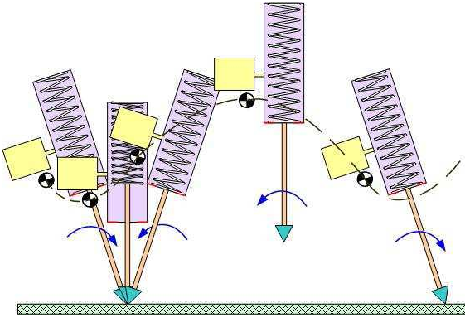
\includegraphics[width=\textwidth]{fig/SLOM_motion.pdf}
\caption{SLOM motion}
\end{figure}

\column{0.5\textwidth}
\begin{block}{Stages}
\begin{itemize}
\item
Lift-off\\[0.1in]
\item
Free fall\\[0.1in]
\item
Touch-down\\[0.1in]
\item
Stance
\end{itemize}
\end{block}
\begin{block}{Terms}
\begin{itemize}
\item
Energy Pumping Mechanism\\[0.1in]
\item
Constraint\\[0.1in]
\item
Energy Release\\[0.1in]
\end{itemize}
\end{block}

\end{columns}
\end{frame}

\subsection*{Aims}
\begin{frame}
\uncover<1->
{
\begin{block}{Design of robot}
\begin{itemize}
  \item Efficient EPM\\[0.1in]
  \item Reaction wheel\\[0.1in]
  \item Onboard electronics
\end{itemize}
\end{block}
}
\uncover<2->
{
\begin{block}{Theory}
\begin{itemize}
  \item Non-linear model\\[0.1in]
  \item Initial conditions\\[0.1in]
  \item In-place hopping\\[0.1in]
  \item Running gait
\end{itemize}
\end{block}
}
\uncover<3->
{
\begin{block}{Experiments}
\begin{itemize}
  \item Attitude estimation\\[0.1in]
  \item Fabrication and interfacing of electronics
\end{itemize}
\end{block}
}
\end{frame}


\section{Design}
\subsection*{Final Design}

\begin{frame}
\frametitle{Final Design}

\begin{columns}

\column{0.5\textwidth}
\begin{figure}
\centering
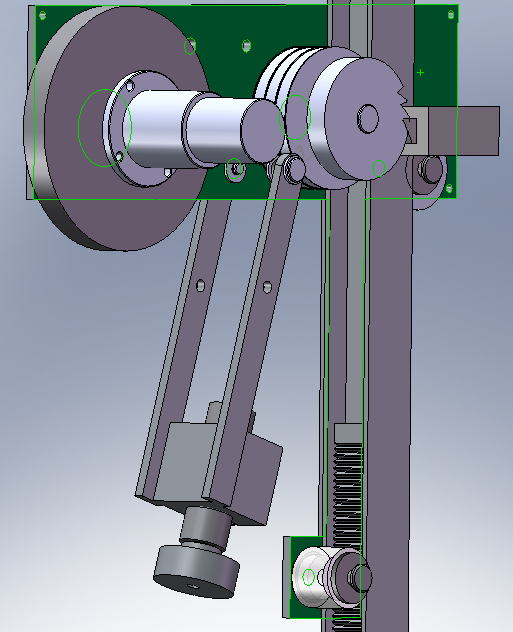
\includegraphics[width=\textwidth]{fig/hopper_detach.png}
\caption{Detached motor sleeve}
\end{figure}

\column{0.5\textwidth}
\begin{block}{Features}
\begin{itemize}
\item
{\greencol EPM :}\\[0.1in]
    \begin{itemize}
    \item
    Motor travels down on rack\\[0.1in]
    \item
    Dual springs, helical gears and slant rack\\[0.1in]
    \end{itemize}
\item
{\greencol Constraint :}\\[0.1in]
    \begin{itemize}
    \item
    Ratchet and Paul\\[0.1in]
    \item
    Band drive\\[0.1in]
    \item
    Disengage motor sleeve\\[0.1in]
    \end{itemize}
\end{itemize}
\end{block}
\end{columns}
\end{frame}

\begin{frame}
\begin{columns}
\column{0.5\textwidth}
\begin{figure}
\centering
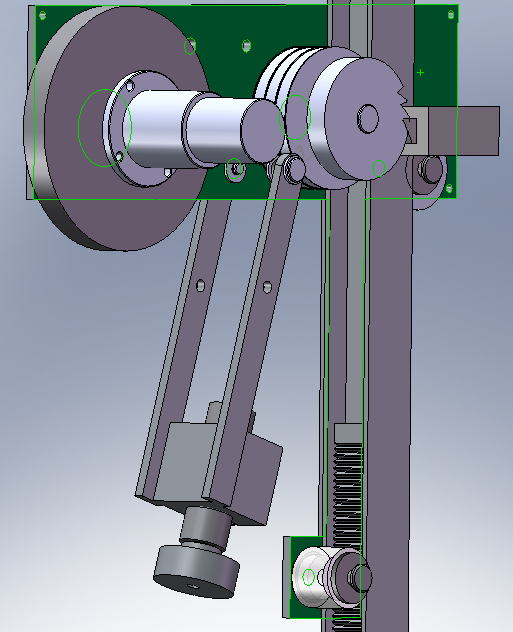
\includegraphics[width=\textwidth]{fig/hopper_detach.png}
\caption{Detached motor sleeve}
\end{figure}

\column{0.5\textwidth}
\begin{figure}
\centering
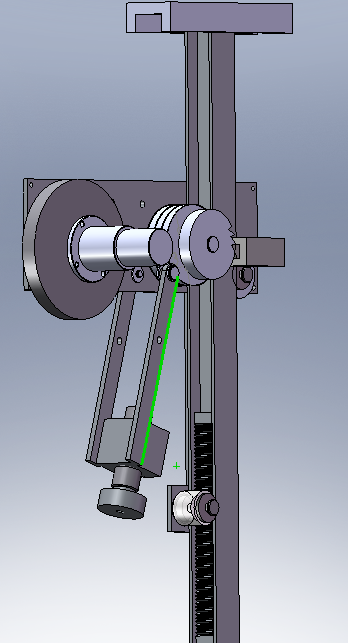
\includegraphics[scale = 0.4]{fig/hopper_bot.png}
\caption{Full Robot}
\end{figure}
\end{columns}
\end{frame}


\begin{frame}
\frametitle{Final Design}
\begin{columns}

\column{0.5\textwidth}
\begin{figure}
\centering
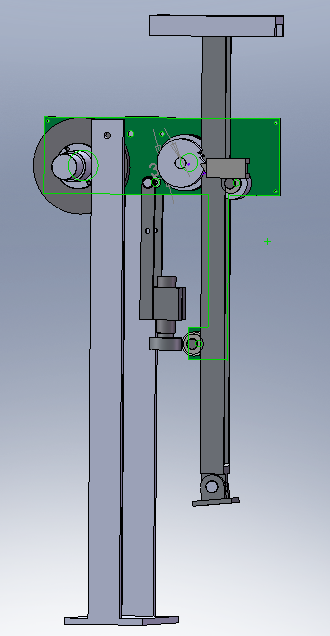
\includegraphics[scale=0.4]{fig/hopper_iso.png}
\caption{Test Rig}
\end{figure}

\column{0.5\textwidth}
\begin{block}{Features}
\begin{itemize}
\item
{\greencol Test-rig :}\\[0.1in]
    \begin{itemize}
    \item
    Pivoted near the C.G.\\[0.1in]
    \item
    Attitude re--orientation\\[0.1in]
    \item
    Simulated hopping\\[0.1in]
    \end{itemize}
\item
{\greencol Overall :}\\[0.1in]
    \begin{itemize}
    \item
    Height : $\sim$ 500 mm\\[0.1in]
    \item
    Leg $\sim$ 0.7 kg\\[0.1in]
    \item
    Total $\sim$ 4.7 kg\\[0.1in]
    \item
    Disengage motor sleeve\\[0.1in]
    \end{itemize}
\end{itemize}
\end{block}
\end{columns}
\end{frame}
\section[Analysis]{Analysis}
\begin{frame}
\frametitle{Objectives}
\begin{block}{Objective}
\begin{itemize}
\item
Estimate masses, dimensions
\item
Choose motors and electronics
\end{itemize}
\end{block}

\begin{columns}
\uncover<1->{
\column{0.5\textwidth}
\vspace*{0.2in}
\begin{block}{Design 1}
\end{block}
\begin{itemize}
\item
Reaction wheel
\item
Springs
\item
Winding motor
\item
Platform
\item
\alert{ Lower leg, main leg masses}
\end{itemize}
}
\uncover<2->{
\column{0.5\textwidth}
\begin{block}{Design 2}
\end{block}
\begin{itemize}
\item
Reaction wheel
\item
Springs
\item
\alert{Rack-pinion drive and motor}
\item
Platform and leg mass
\end{itemize}
}
\end{columns}
\end{frame}

\subsection*{Two Mass Problem}
\begin{frame}
\frametitle{Two Mass Problem}

\begin{columns}
\column{0.4\textwidth}

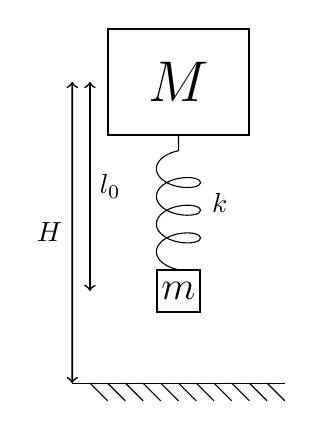
\begin{tikzpicture}[scale=0.45]
\draw (-3,0) -- (3,0);
\foreach \x in {-2.5,-2,...,2.5}
\draw (\x,0) -- (\x+0.5,-0.5);
\path (-2,7) coordinate(M1);
\path (2,10) coordinate(M2);
\path (-0.6,2) coordinate(m1);
\path (0.6,3.2) coordinate(m2);
\draw [thick](M1) rectangle (M2) node[midway]{\huge{$M$}};
\draw [thick](m1) rectangle (m2) node[midway]{\Large{$m$}};
\path (-2.5,0) coordinate (O);
\path (-2.5,2.6) coordinate (SPL);
\path (-2.5,8.5) coordinate (H);
\draw[<->] [semithick](O)++(-0.5,0) -- (-3,8.5) node[midway, left]{$H$};
\draw[<->] [semithick](SPL) -- (H) node[midway, right]{$l_0$};
\draw[snake=coil, segment amplitude=8pt] (0,3.2) -- (0,7) node[midway,right=2ex]{$k$};
\end{tikzpicture}

\column{0.6\textwidth}
\uncover<1->{
\begin{itemize}
\item
\begin{equation*}
h_n = \frac{Mh_{n-1} + ml_0}{M + m}
\end{equation*}
\item
\begin{equation*}
E_{loss} = \frac{Mg\;(H-l_0)}{1 + M/m}
\end{equation*}
\end{itemize}
}

\visible<2->{
\begin{figure}
\centering
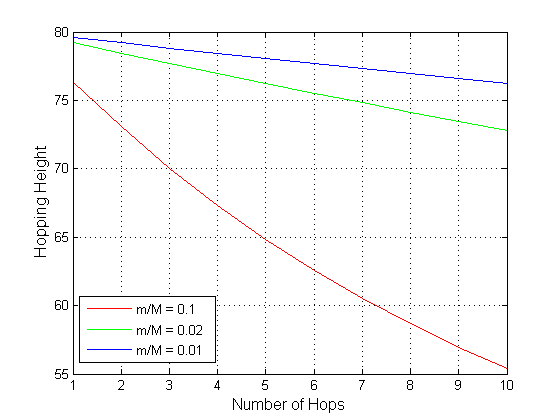
\includegraphics[scale=0.4]{fig/hopHeight.png}
\end{figure}
}
\end{columns}

\end{frame}

\begin{frame}
\frametitle{Torque Requirements}
\begin{columns}
\column{0.7\textwidth}
\begin{figure}
\centering
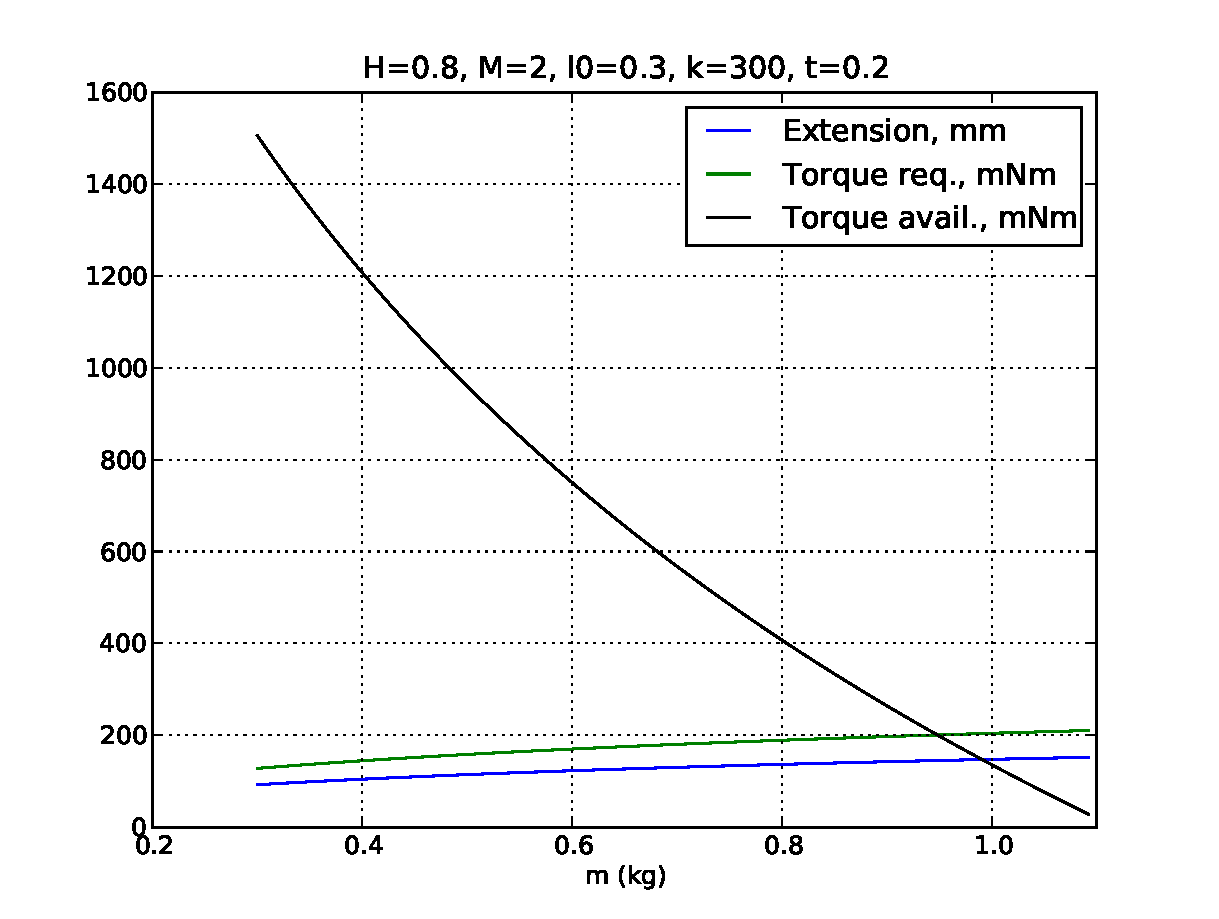
\includegraphics[width=\textwidth]{fig/2mass.pdf}
\end{figure}

\column{0.4\textwidth}
\visible<2->{
\begin{block}{Results}
\begin{itemize}
\item
m $\sim$ 0.5 kg
\item
k $\sim$ 300 N
\item
M $\sim$ 2 kg
\item
Lower leg $\sim$ 12 cms
\item
Standard rack-pinion
\item
Faulhabeur 2342 motor
\item
43 : 1 gearbox
\end{itemize}
\end{block}
}
\end{columns}
\end{frame}


\subsection*{Reaction Wheel}
\begin{frame}
\frametitle{ReWac : Idea and Advantages}
\begin{columns}

\column{0.4\textwidth}
\begin{figure}
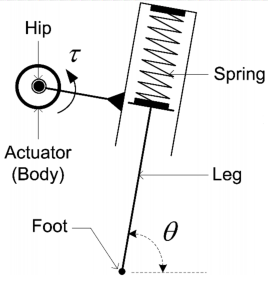
\includegraphics[width=\textwidth]{fig/slom.pdf}
\caption{ReWac : Schematic}
\end{figure}

\column{0.6\textwidth}
\begin{block}{Inertia Wheel Assembly}
Conserve angular momentum
\begin{equation*}
\dot{\theta}_b = -\frac{J_{w}}{J_{b}+J_{w}}\dot{\theta}_w
\end{equation*}
\end{block}

\vspace{0.5in}
\begin{block}{Uses}
\begin{itemize}
\item
Initial condition\\[0.1in]
\item
Changing hopping height online\\[0.1in]
\item
Change from an \alert{arbitrary} pitch to \alert{steady state} pitch
within one hop
\end{itemize}
\end{block}
\end{columns}

\end{frame}

\begin{frame}
\frametitle{ReWac : Radius}
\begin{figure}
\centering
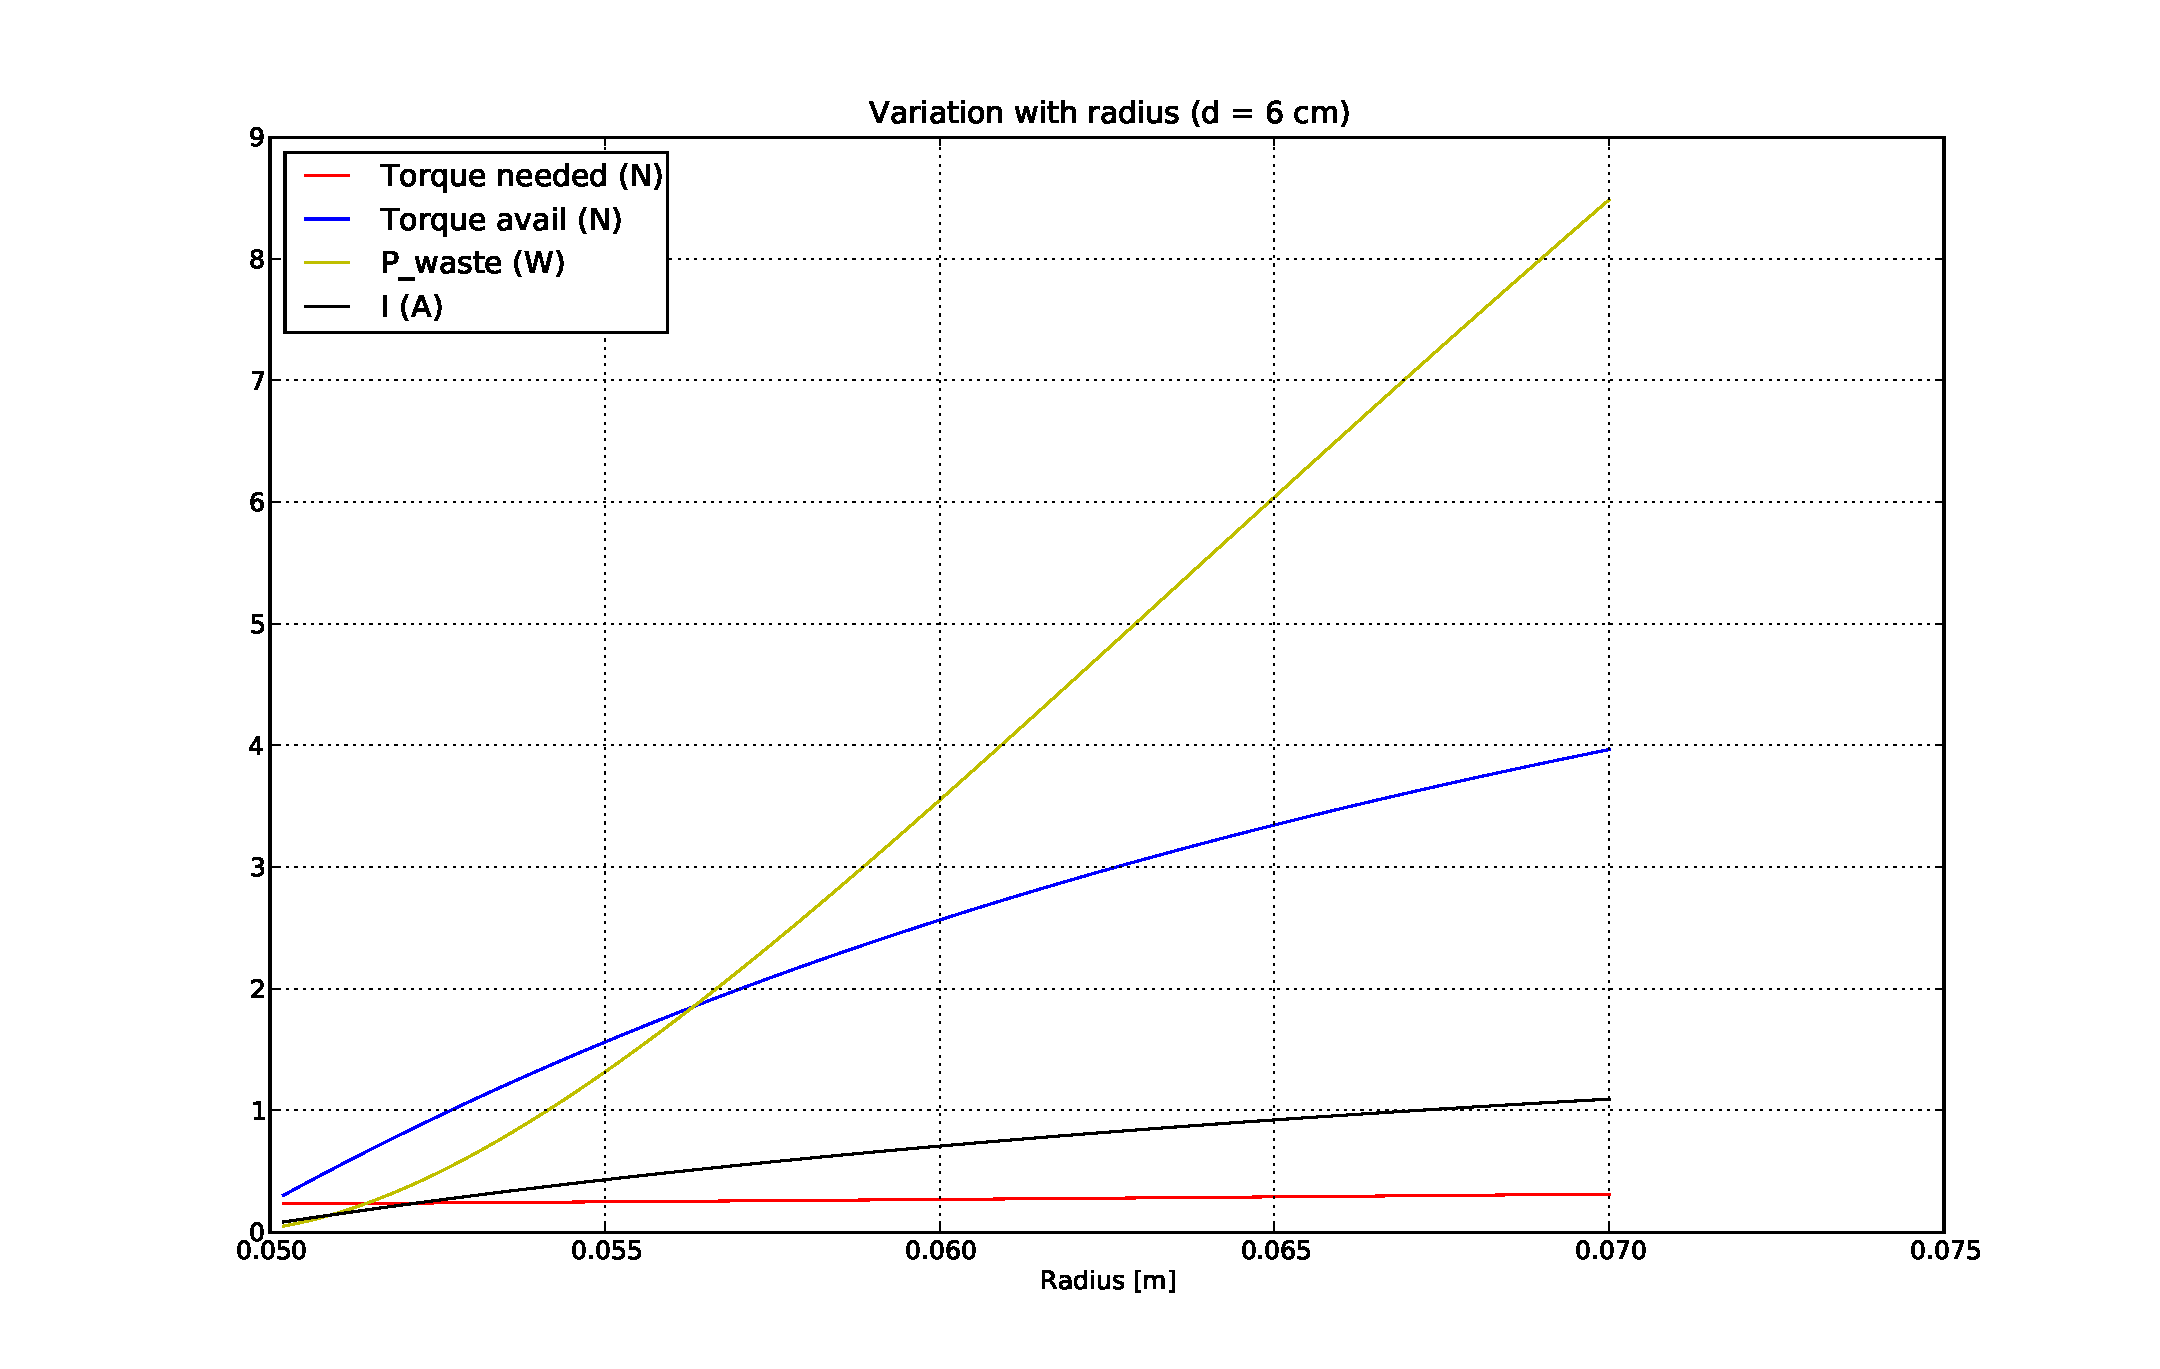
\includegraphics[width=\textwidth]{fig/rewac_radius.pdf}
\end{figure}
\end{frame}

\begin{frame}
\frametitle{ReWac : CG distance}
\begin{figure}
\centering
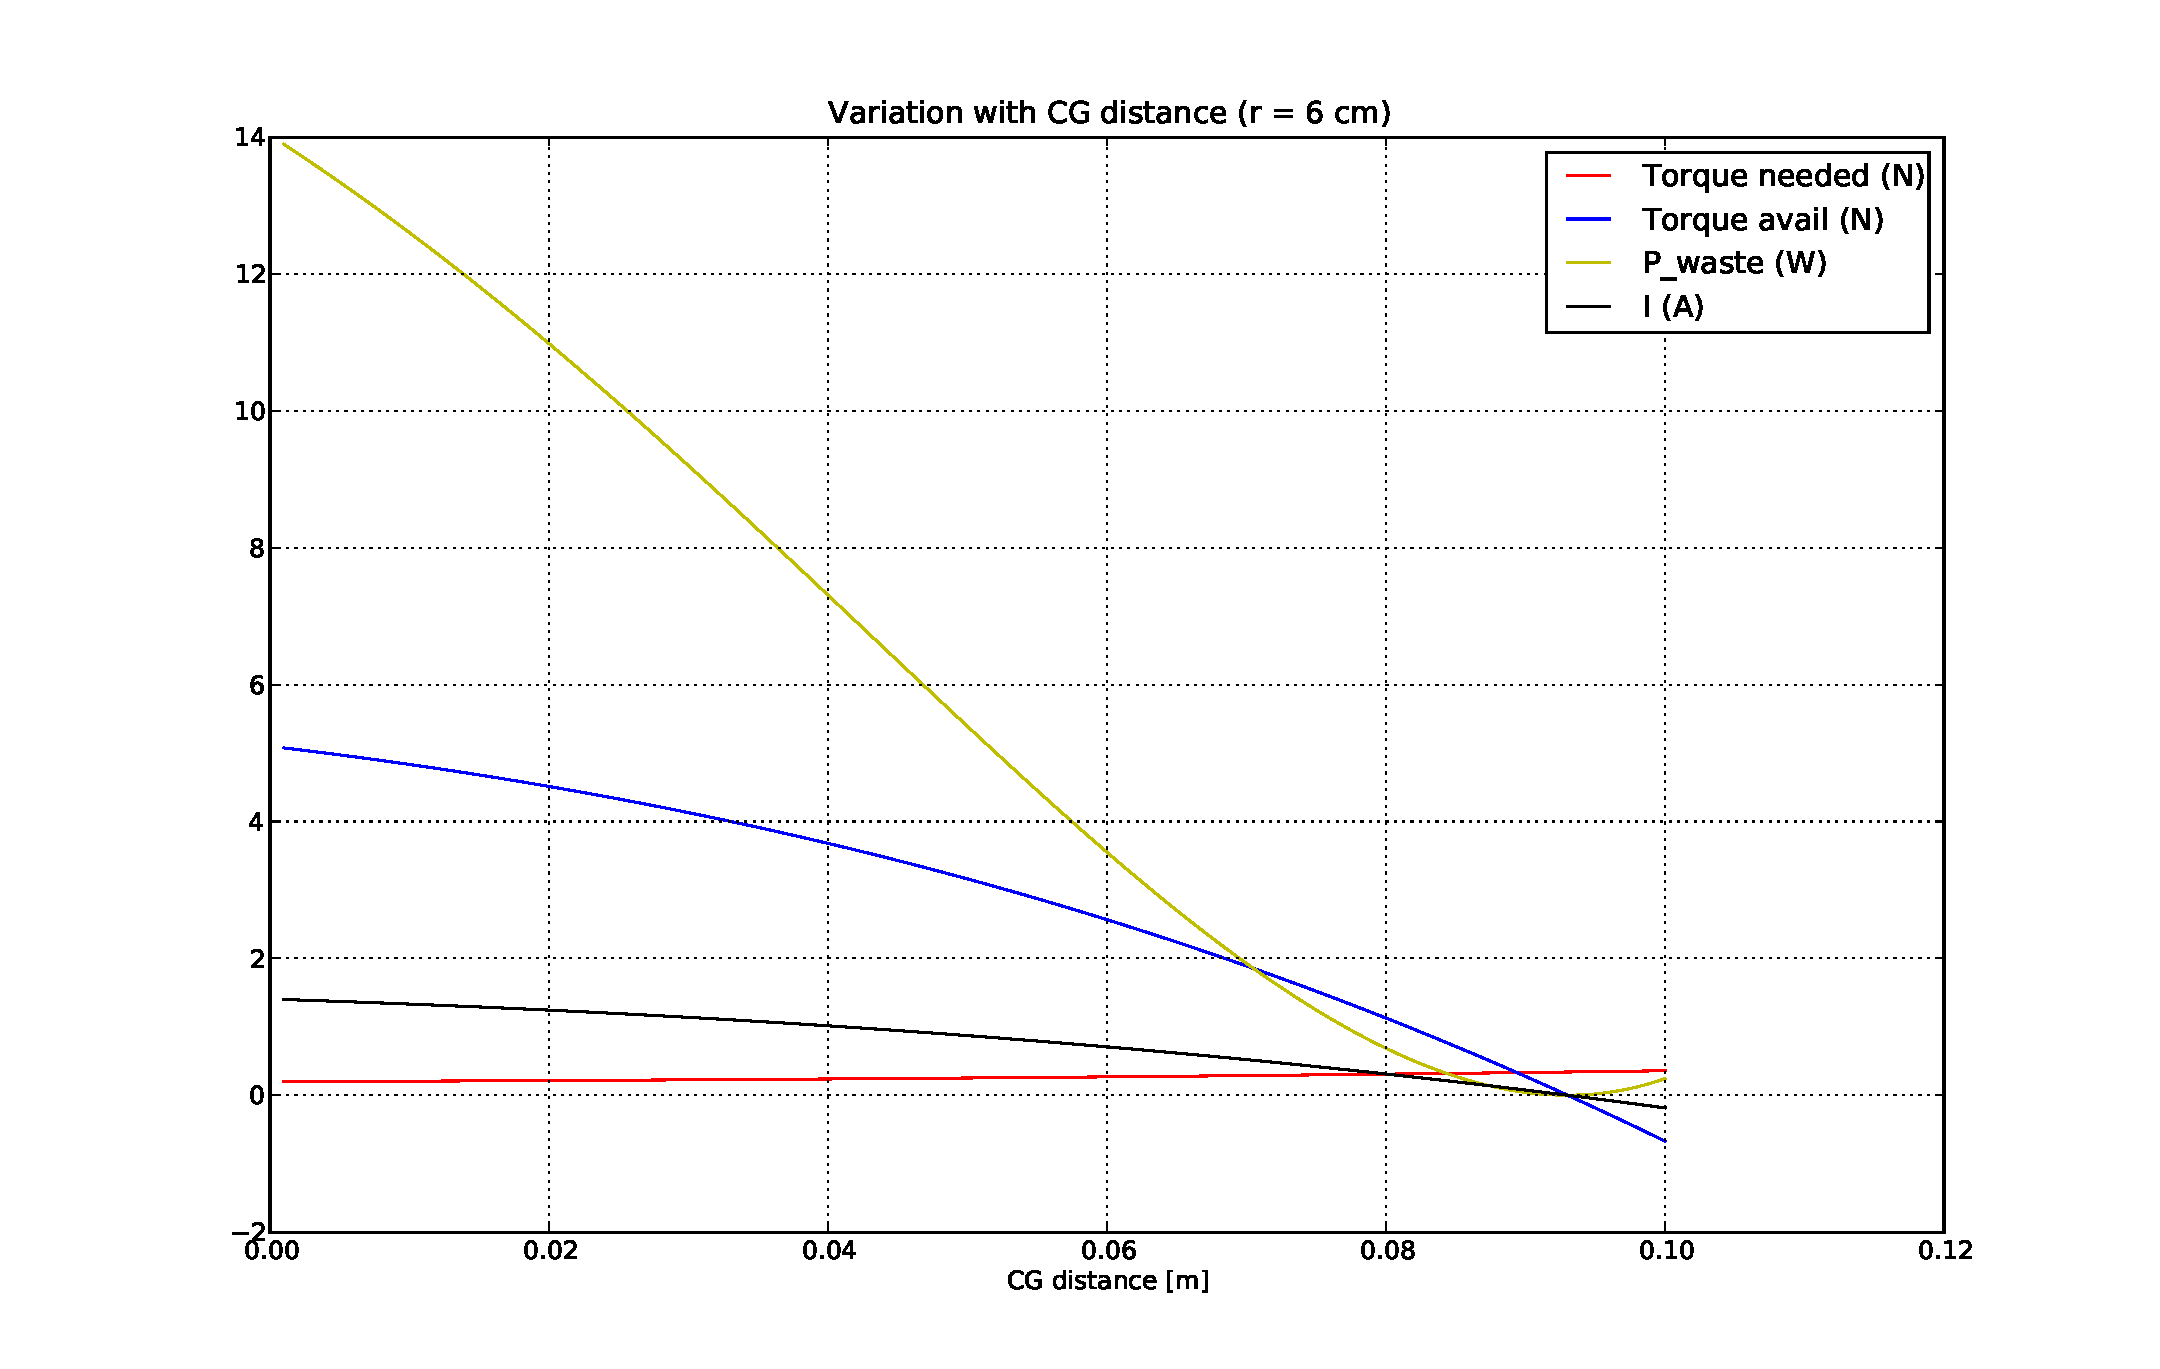
\includegraphics[width=\textwidth]{fig/rewac_dist.pdf}
\end{figure}
\end{frame}

\subsection*{Impact Analysis}
\begin{frame}
\frametitle{Impact Analysis}
\uncover<1->{
\begin{block}{Concept}
\begin{itemize}
\item
Desired hopping height dictates impact frequency\\[0.2in]
\item
Masses dictate energy loss\\[0.2in]
\item
\alert{Natural frequency} of the system should be much \alert{higher} than hopping frequency\\[0.2in]
\end{itemize}
\end{block}
}
\uncover<2->{
\begin{block}{Results}
\begin{itemize}
\item
Hopping frequency is a weak function of hopping height and M\\[0.2in]
\item
A large \alert{dependence} on \alert{leg mass}
\end{itemize}
\end{block}
}
\end{frame}

\begin{frame}
\frametitle{Impact : Leg mass}
\begin{figure}
\centering
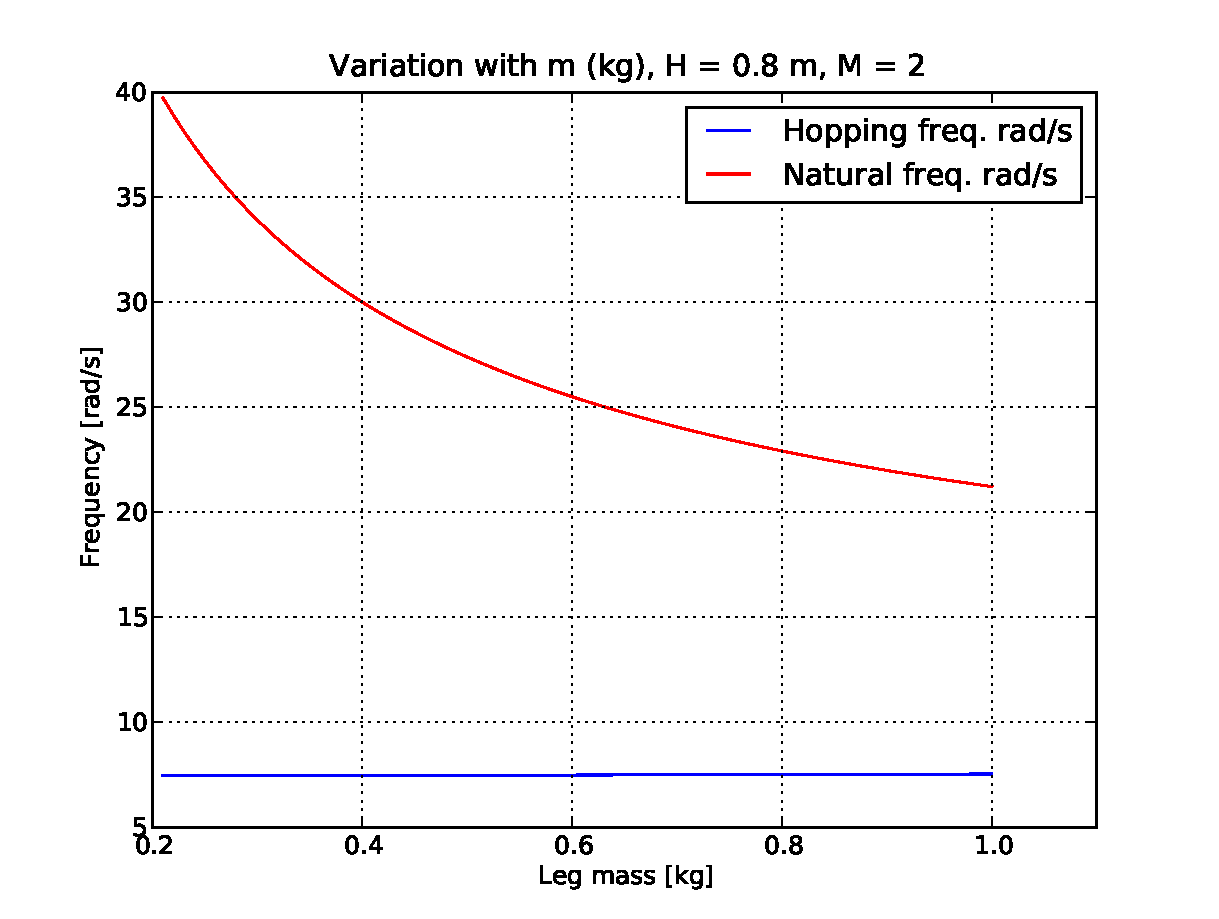
\includegraphics[width=\textwidth]{fig/freq_smallM.pdf}
\end{figure}
\end{frame}


\section{Embedded System}
\subsection*{Hardware}
\begin{frame}
\frametitle{ReWac Board Hardware}
    \begin{columns}
        \column{0.6\textwidth}
        \begin{figure}
        \centering
        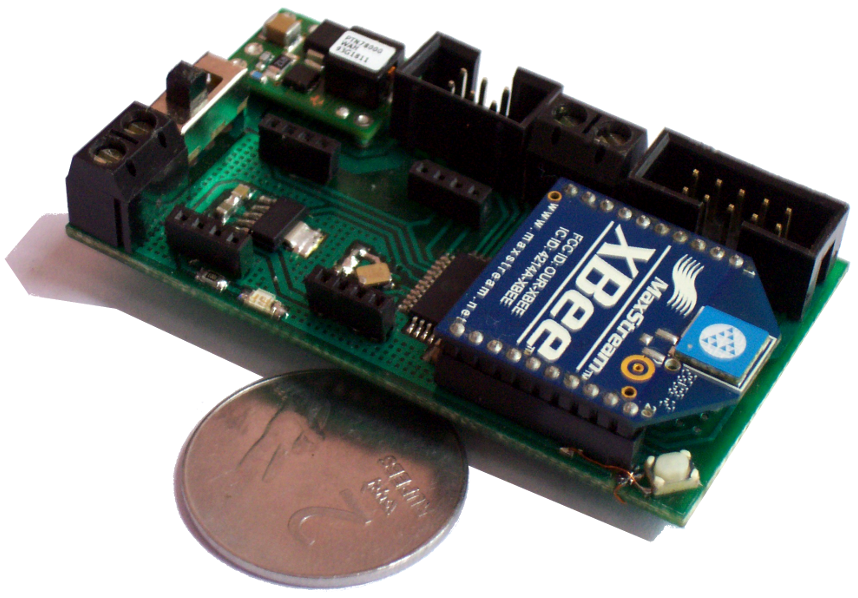
\includegraphics[scale=0.2]{fig/rewac.png}
        \end{figure}
        
        \column{0.4\textwidth}
        \begin{itemize}
        \item
        Microchip dsPIC33F\\[0.05in]
        40 MIPS\\[0.1in]
        \item
        Accelerometer\\[0.05in]
        2.162 LSB/mg\\[0.1in]
        \item
        Gyroscope (50 Hz)\\[0.05in]
        0.07326 $^o/s/$LSB\\[0.1in]
        \item
        Quadrature Encoders\\[0.1in]
        \item
        XBee module\\[0.1in]
        \end{itemize}
    \end{columns}
\end{frame}

\subsection*{Kalman Filter}
\begin{frame}
\frametitle{Kalman Filter}
\begin{block}{Why}
\begin{itemize}
\item
Pitch attitude estimate
\item
Computing power
\end{itemize}
\end{block}

\begin{block}{How}
\begin{equation*}
\bm{x} = [x_1\;\;x_2]^T = [\theta\;\;\dot{\theta}]^T
\end{equation*}
\vspace{0.075in}
\begin{equation*}
\bm{x}_{k+1} = \bm{A}\:\bm{x}_k + \bm{B}\:\bm{u}_k + \bm{w}_k
\end{equation*}
\vspace{0.075in}
\begin{equation*}
y_{k+1} = \bm{C}\:\bm{x}_{k+1} + z_{k+1}
\end{equation*}
\end{block}

\begin{block}{Tricks}
\begin{itemize}
\item
\alert{Sparse covariance matrix}
\item
Remove matrix operations
\item
\alert{Fixed point arithmetic}
\end{itemize}
\end{block}
\end{frame}

\begin{frame}
\frametitle{Attitude Estimation}

\begin{columns}

\column{0.5\textwidth}

\begin{block}{Accelerometer}
\begin{itemize}
\item
Slow, absolute reading
\item
\alert{Body accelerations} - Noise
\item
High frequency noise
\end{itemize}
\end{block}

\begin{block}{Gyroscope}
\begin{itemize}
\item
Fast
\item
Drifts slowly, randomly
\end{itemize}
\end{block}

\column{0.5\textwidth}
\begin{itemize}
    \item
    After liftoff $\sim$ { \greencol 250 ms}\\[0.1in]
    \begin{itemize}
        \item
        Only force is gravity\\[0.1in]
        \item
        Both sensors used\\[0.2in]
    \end{itemize}

    \item
    Free fall $\sim$ {\greencol 250 ms}\\[0.1in]
    \begin{itemize}
        \item
        No accelerometer reading\\[0.1in]
        \item
        Propagate using rate only\\[0.2in]
    \end{itemize}

    \item
    Stance $\sim$ {\greencol 150 ms}\\[0.1in]
    \begin{itemize}
        \item
        \alert{Ankle potentiometer}
    \end{itemize}

\end{itemize}
\end{columns}
\end{frame}

\begin{frame}
\frametitle{High Frequency Input sampled at 50 Hz}
\begin{figure}
\centering
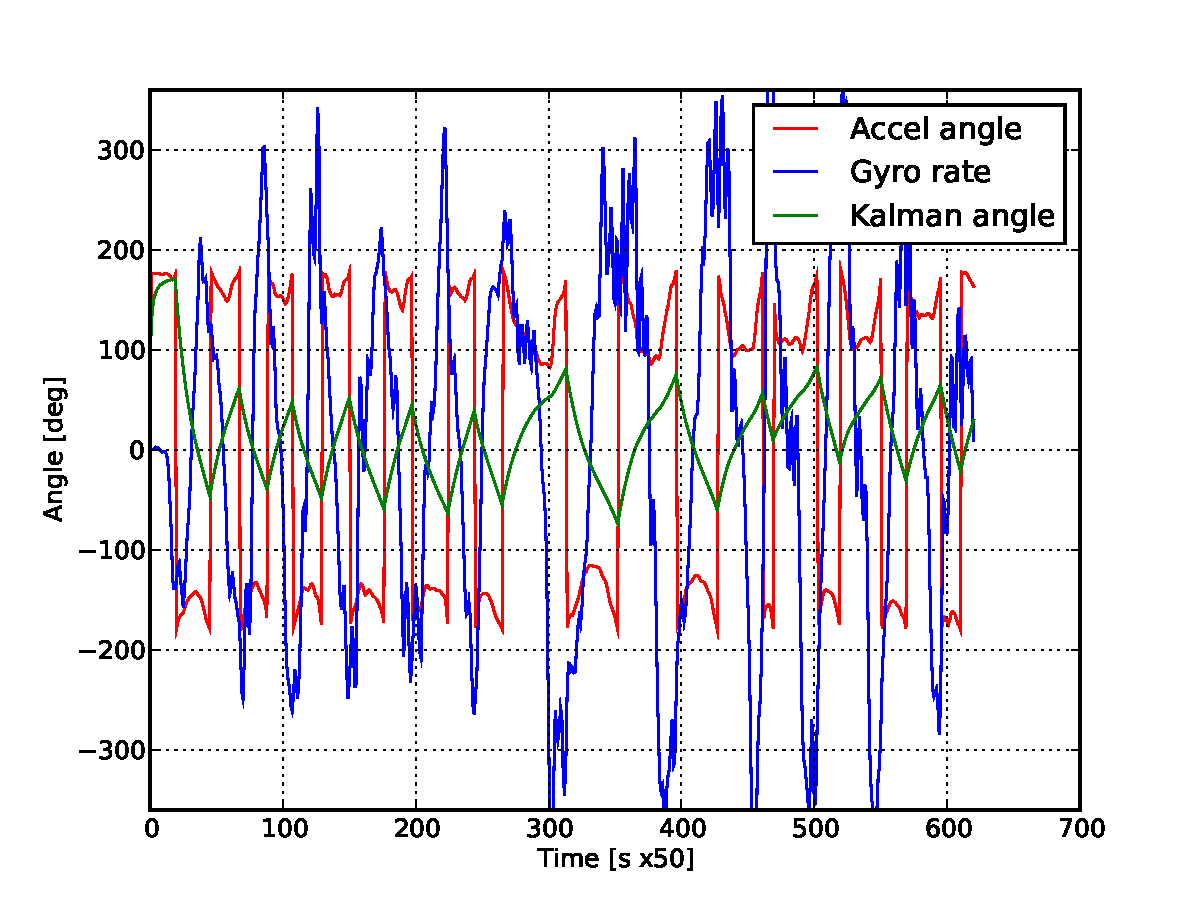
\includegraphics[width=\textwidth]{fig/kf.pdf}
\end{figure}
\end{frame}


\end{document}


